% Verbatim source: Report/initial/Logistic Regression with References.docx
\addsec{\src{Alternative Model: Logistic Regression}}

\src{To evaluate an alternative to the random forest, we used a logistic regression model to predict whether an IMF lending program would be interrupted. We chose logistic regression because the dependent variable, \emph{interrupted}, is binary (Hosmer et al., 2013, p. 1; James et al., 2013, pp. 130–131). It provides a relatively simple and interpretable benchmark against which the performance of a more complex model can be analyzed.}

\src{The model was trained on the same 13 explanatory variables as the random forest, covering program design, conditionality, previous program experience and macroeconomic conditions. These include economic growth, inflation, whether an arrangement is extended or concessional, and the number of prior actions required before approval. The model estimates the probability of an interruption, which is converted into a binary prediction using a threshold of 0.50 (James et al., 2013, p. 146). It was not tuned, while the random forest was tuned and its threshold searched out of fold. The same training and test sets were used for both models, allowing a direct comparison.}

\src{On the test set of 28 programs, logistic regression achieved an accuracy of 0.536, a balanced accuracy of 0.570 and an AUC of 0.684, against 0.500, 0.508 and 0.586 for the random forest at its selected threshold of 0.51. At the same 0.50 threshold, however, the forest reaches 0.571 and 0.567, so the two models differ mainly in AUC, which does not depend on the threshold (Fawcett, 2006): logistic regression ranks interrupted programs above completed ones more consistently. With 28 test programs, even this gap should be read cautiously, and both results show that predicting interruptions remains difficult.}

\src{A key advantage of logistic regression is its interpretability. Its coefficients indicate how each explanatory variable is associated with the log-odds of interruption, holding the other variables constant (Hosmer et al., 2013, pp. 49–52; see Figure 1). The largest coefficients belong to extended facilities (−4.18, \emph{p} = .004) and concessional facilities (2.31, \emph{p} = .087), of which only the former is statistically significant at the 5\% level. These two variables are strongly correlated in the training data (\emph{r} = .81). As a result, the model splits their joint association into opposite signs and estimates both with large standard errors, so their individual coefficients should not be read in isolation (James et al., 2013, pp. 99–102). The absence of a track record also has a sizeable positive coefficient (1.31), but it is imprecisely estimated (\emph{p} = .231). More generally, these associations are not causal, and coefficient magnitudes are not directly comparable because the predictors are measured on different scales (Hosmer et al., 2013, pp. 62–64).}

\begin{wordtable}
\wordcaption{\src{Figure 1}\par
\src{\emph{Logistic Regression Coefficients for Program Interruption}}}
{\centering
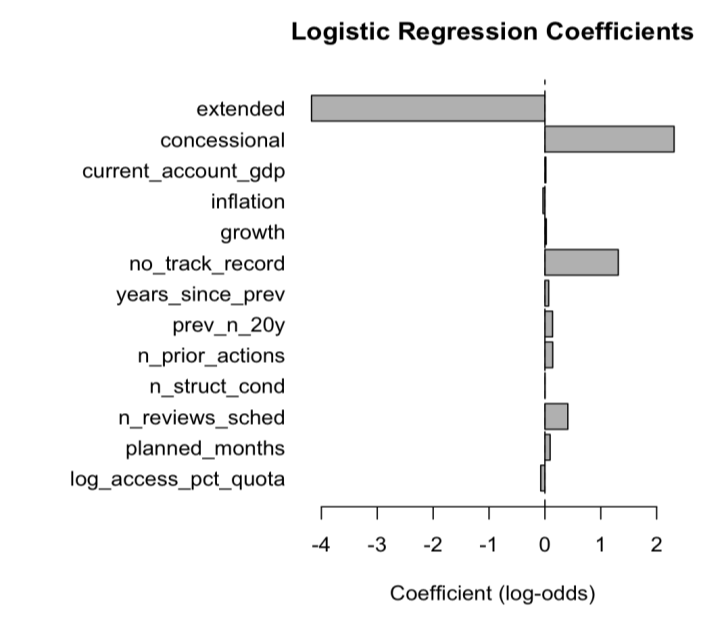
\includegraphics[width=0.78\linewidth]{../Presentation/figures/logit_coefficients.png}\par}
\smallskip
{\footnotesize\src{\emph{Note.} Coefficients are in log-odds and estimated on the training set. Positive values indicate higher odds of interruption. Predictors are on different scales, so bar lengths are not directly comparable measures of importance. Extended and concessional are strongly correlated (\emph{r} = .81).}\par}
\end{wordtable}

\src{The random forest, in contrast, can capture non-linear relationships and interactions between variables (Breiman, 2001a), at the cost of interpretability (Breiman, 2001b; James et al., 2013, pp. 24–26). Logistic regression imposes a simpler functional form and provides a more transparent account of the relationships it represents.}

\src{Overall, logistic regression matched the random forest on balanced accuracy and ranked programs better, while offering greater interpretability. One possible explanation is that the simpler model generalized better, whereas the random forest’s flexibility may have made it more susceptible to fitting noise in the training data (Hastie et al., 2009, pp. 219–223; James et al., 2013, pp. 33–36). However, this cannot be established from the results alone, and with only 28 test programs the differences should be interpreted cautiously. The comparison shows that a more complex model does not necessarily produce better predictions (Christodoulou et al., 2019; Couronné et al., 2018), and that interpretability remains an important consideration when evaluating models for financial decision-making (Rudin, 2019).}
